\section{Adaptive IPC Framework and Kernel Module}
\label{sec:adaptive_kernel}

This section describes the mathematical formulation of the adaptive IPC selection policies, the closed-loop EWMA telemetry controller, and the architectural design of the custom Linux kernel mailbox module.

\subsection{Payload-Based Transport Selection}
Different IPC mechanisms exhibit distinct overhead characteristics depending on payload size. For small messages, system-call transition overhead and buffer copying dominate execution time; for large messages, memory copy bandwidth and buffer exhaustion govern latency.

To capture this relationship, we formulate an empirical oracle selector. Let $\mathcal{M} = \{\text{pipe}, \text{fifo}, \text{sysv}, \text{posix}, \text{shm}, \text{uds}\}$ denote the set of available IPC transports, and let $\mathcal{S}$ denote the discrete set of payload sizes. The empirical best transport $m^*(s)$ for payload size $s$ is defined as:
\begin{equation}
m^*(s) = \arg\min_{m \in \mathcal{M}} L(m, s)
\end{equation}
where $L(m, s)$ represents the mean round-trip latency of transport $m$ transferring a payload of $s$ bytes.

\begin{figure*}[!t]
\centering
\subfloat[Adaptive Transport Selection Decision Flowchart]{\begin{tikzpicture}[
    scale=0.72, every node/.style={transform shape},
    startstop/.style={draw=black!70, fill=red!10, rounded corners=2pt, font=\scriptsize\bfseries, minimum height=0.6cm, align=center},
    decision/.style={diamond, draw=black!70, fill=orange!15, font=\scriptsize, aspect=1.8, inner sep=2pt, align=center},
    block/.style={draw=black!70, fill=blue!10, rounded corners=2pt, font=\scriptsize, minimum height=0.6cm, align=center},
    arr/.style={->, >=stealth, thick, draw=black!70}
]

\node[startstop] (start) at (3.8, 4.3) {Message Payload $s$};
\node[decision] (check_size) at (3.8, 3.2) {$s > 1,024\text{ B}$?};
\node[block] (pipe_route) at (6.8, 3.2) {Route to \textbf{PIPE}\\ \scriptsize ($s > \text{SHM Limit}$)};

\node[decision] (check_ctrl) at (3.8, 1.8) {EWMA Active?};
\node[decision] (check_hyst) at (1.4, 0.5) {$\bar{L}(\text{SHM}) > 1.08 \bar{L}(\text{PIPE})$?};

\node[block] (static_shm) at (6.0, 1.8) {Route to \textbf{SHM}\\ \scriptsize ($s \le 1,024\text{ B}$)};

\node[block] (switch_pipe) at (-0.2, -0.8) {Switch \textbf{PIPE}\\ \scriptsize Increment switches};
\node[block] (stay_shm) at (3.0, -0.8) {Retain / Switch \textbf{SHM}\\ \scriptsize Zero futex copy};

\draw[arr] (start) -- (check_size);
\draw[arr] (check_size) -- node[above, font=\tiny] {Yes} (pipe_route);
\draw[arr] (check_size) -- node[right, font=\tiny] {No} (check_ctrl);
\draw[arr] (check_ctrl) -- node[above, font=\tiny] {No} (static_shm);
\draw[arr] (check_ctrl) -| node[above, font=\tiny] {Yes} (check_hyst);
\draw[arr] (check_hyst) -| node[left, font=\tiny] {Yes} (switch_pipe);
\draw[arr] (check_hyst) -| node[right, font=\tiny] {No} (stay_shm);

\end{tikzpicture}
\label{fig:adaptive_selector}}
\hfil
\subfloat[Custom Linux Kernel Mailbox Architecture (\texttt{/dev/aipc})]{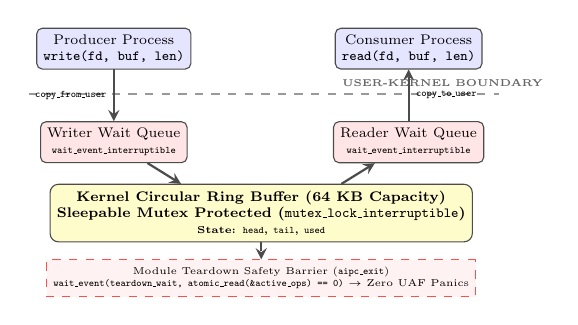
\begin{tikzpicture}[
    scale=0.72, every node/.style={transform shape},
    box/.style={draw=black!70, fill=blue!10, rounded corners=2pt, font=\scriptsize, align=center, minimum height=0.6cm},
    kbox/.style={draw=black!70, fill=red!10, rounded corners=2pt, font=\scriptsize, align=center, minimum height=0.6cm},
    ring/.style={draw=black!70, fill=yellow!20, rounded corners=3pt, font=\scriptsize\bfseries, align=center, minimum width=6.0cm, minimum height=0.9cm},
    barrier/.style={draw=red!70, fill=red!5, dashed, font=\tiny, align=center, minimum width=6.0cm, minimum height=0.65cm},
    arr/.style={->, >=stealth, thick, draw=black!70}
]

% Userspace processes
\node[box, minimum width=2.4cm] (writer) at (0, 3.2) {Producer Process\\ \scriptsize \texttt{write(fd, buf, len)}};
\node[box, minimum width=2.4cm] (reader) at (5.2, 3.2) {Consumer Process\\ \scriptsize \texttt{read(fd, buf, len)}};

% Kernel Boundary
\draw[thick, dashed, draw=black!40] (-1.5, 2.4) -- (6.8, 2.4);
\node[font=\tiny\bfseries, text=black!60] at (5.8, 2.6) {USER-KERNEL BOUNDARY};

% Wait Queues
\node[kbox, minimum width=2.4cm] (wq_write) at (0, 1.55) {Writer Wait Queue\\ \tiny \texttt{wait\_event\_interruptible}};
\node[kbox, minimum width=2.4cm] (wq_read) at (5.2, 1.55) {Reader Wait Queue\\ \tiny \texttt{wait\_event\_interruptible}};

% Mutex & Ring Buffer
\node[ring] (rb) at (2.6, 0.3) {Kernel Circular Ring Buffer (64 KB Capacity)\\ \scriptsize Sleepable Mutex Protected (\texttt{mutex\_lock\_interruptible})\\ \tiny State: \texttt{head}, \texttt{tail}, \texttt{used}};

% Teardown barrier
\node[barrier] (teardown) at (2.6, -0.85) {Module Teardown Safety Barrier (\texttt{aipc\_exit})\\ \tiny \texttt{wait\_event(teardown\_wait, atomic\_read(\&active\_ops) == 0)} $\to$ Zero UAF Panics};

% Connecting Arrows
\draw[arr] (writer) -- node[left, font=\tiny] {\texttt{copy\_from\_user}} (wq_write);
\draw[arr] (wq_write) -- (rb.160);
\draw[arr] (rb.20) -- (wq_read);
\draw[arr] (wq_read) -- node[right, font=\tiny] {\texttt{copy\_to\_user}} (reader);
\draw[arr, dashed] (rb) -- (teardown);

\end{tikzpicture}
\label{fig:kernel_mailbox}}
\caption{Adaptive Telemetry Control and Kernel Mailbox Subsystems: (a) Decision logic enforcing payload threshold boundaries, EWMA telemetry evaluation, and an 8\% hysteresis switching band; and (b) Kernel character device architecture featuring a 64 KB circular ring buffer, sleepable mutex synchronization, blocking wait queues, and an atomic teardown barrier.}
\label{fig:adaptive_and_kernel}
\end{figure*}

The \textbf{Latency Regret} incurred by selecting transport $m$ instead of optimal transport $m^*(s)$ is $R_{\text{lat}}(s) = L(m, s) - L(m^*(s), s)$, expressed as a percentage: $R_{\text{lat, \%}}(s) = \frac{L(m, s) - L(m^*(s), s)}{L(m^*(s), s)} \times 100\%$.
The overall \textbf{Selection Accuracy} of an adaptive policy across all evaluated payload sizes $\mathcal{S}$ is:
\begin{equation}
\text{Accuracy} = \frac{1}{|\mathcal{S}|} \sum_{s \in \mathcal{S}} \mathbf{1}\left(m_{\text{selected}}(s) = m^*(s)\right) \times 100\%
\end{equation}

\subsection{EWMA-Based Telemetry Controller and Hysteresis}
Static size thresholds cannot adapt to transient runtime contention or host virtualization pauses. To achieve closed-loop adaptation, Mini-A-IPC implements an Exponentially Weighted Moving Average (EWMA) latency tracking controller in \texttt{src/selector.c}. 
Upon each completed message exchange, the controller updates the smoothed latency estimate $\bar{L}^{(t)}$ for active transport $m$:
\begin{equation}
\bar{L}^{(t)}_m = \alpha \cdot L_{\text{sample}} + (1 - \alpha) \cdot \bar{L}^{(t-1)}_m
\end{equation}
where $\alpha = 0.15$ is the empirical smoothing factor, chosen to balance responsiveness to genuine phase shifts against resilience to transient measurement spikes.

Under noisy multi-tenant execution, adjacent transports with comparable mean latencies can oscillate rapidly (flapping), incurring prohibitive reconfiguration costs. To prevent thrashing, the controller enforces an 8\% hysteresis switching margin ($h = 1.08$): $\text{SHM} \to \text{PIPE}$ requires $\bar{L}_{\text{SHM}} > 1.08 \bar{L}_{\text{PIPE}}$, and $\text{PIPE} \to \text{SHM}$ requires $\bar{L}_{\text{PIPE}} > 1.08 \bar{L}_{\text{SHM}}$.
As detailed in Fig.~\ref{fig:adaptive_and_kernel}(a), payloads $> 1024$~bytes immediately bypass shared memory and route to streaming transports due to the structural capacity boundary of the shared mailbox.

\subsection{Kernel Mailbox Design (\texttt{/dev/aipc})}
To investigate driver-assisted communication without user-space semaphore synchronization, we implemented \texttt{/dev/aipc}, an out-of-tree Linux character device driver (\texttt{kernel/aipc\_module.c}). Fig.~\ref{fig:adaptive_and_kernel}(b) illustrates the driver architecture.
The driver maintains a 64~KB circular ring buffer allocated in kernel memory via \texttt{kmalloc(GFP\_KERNEL)}. Key design features include:
\textbf{1) Sleepable Mutex Synchronization:} Access to the circular buffer indices (\texttt{head}, \texttt{tail}, \texttt{used}) is protected by a Linux kernel mutex (\texttt{struct mutex lock}). Because memory copy operations between user and kernel space (\texttt{copy\_from\_user}, \texttt{copy\_to\_user}) can trigger page faults and sleep, spinlocks cannot be held during data copying. The sleepable mutex safely accommodates page faults without deadlocking the kernel.
\textbf{2) Wait Queue Flow Control:} When the buffer is empty, reader threads suspend on the \texttt{readers} wait queue using \texttt{wait\_event\_interruptible()}. When the buffer is full, writer threads suspend on the \texttt{writers} wait queue. Each successful write wakes blocked readers, and each read wakes blocked writers.
\textbf{3) VFS 6.12+ Compatibility:} Modern Linux kernels (Linux 6.12+) deprecate the legacy \texttt{no\_llseek} file operation pointer. The driver incorporates \texttt{noop\_llseek} to ensure seamless compilation across modern kernels.

\subsection{Teardown Barrier and Memory Safety}
A notorious vulnerability in out-of-tree kernel modules is the Use-After-Free (UAF) race condition during module unloading (\texttt{rmmod}). In unoptimized drivers, executing \texttt{wake\_up\_all()} followed immediately by \texttt{kfree(aipc)} panics the kernel if a waking reader thread accesses the deallocated device structure.
Mini-A-IPC eliminates this defect by implementing an atomic reference-counting teardown barrier: the driver maintains \texttt{atomic\_t active\_ops}, incremented on \texttt{aipc\_open()} and decremented on \texttt{aipc\_release()}. In \texttt{aipc\_exit()}, the driver sets \texttt{shutdown = true} under the mutex lock and wakes sleeping readers and writers with an \texttt{-EPIPE} error. The module unload thread suspends on \texttt{wait\_event(aipc->teardown\_wait, atomic\_read(\&aipc->active\_ops) == 0)}, guaranteeing that \texttt{kfree()} deallocation proceeds only after all open file descriptors have terminated and released driver structures.
